\section{Company Clustering Algorithm}
As already discussed in section \ref{clusteringDiscussion} this thesis will compare the results between a bottom-up
agglomerative hierarchical clustering and the partitional kMeans clustering algorithm, which are both \emph{exclusive}
and \emph{intrinsic}. The clustering and scoring is based on the assumption that \emph{every company raises only one demand}.
This is necessary to simplify the demand prediction and the cluster rating. It does not distort the results respectively
to the correlation of companies' demands and their characteristics.

This section describes where the used data comes from and how it was processed and prepared for clustering. Further more this
section will outline how the proximity between companies were calculated and how the resulting clusters were scored.

\subsection{Data}
To determine clusters of companies, its necessary to have a data-set that contains the relevant information
for a company, and has to be big enough to get meaningful results.

\begin{figure}[ht]
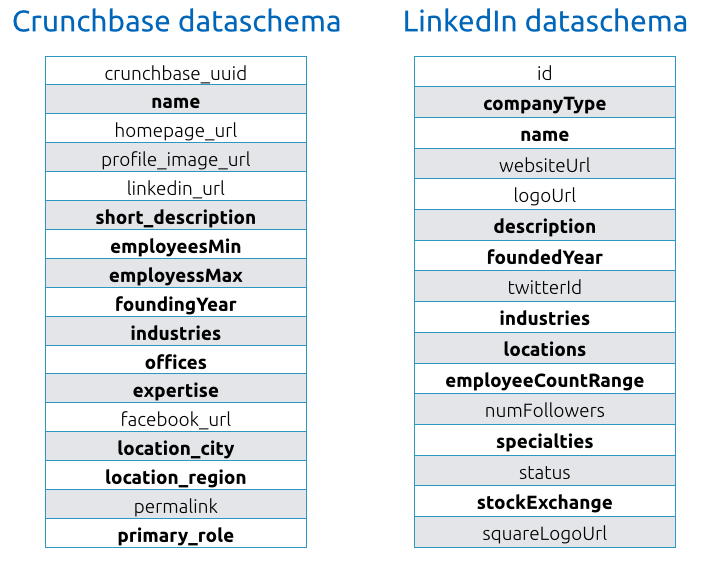
\includegraphics[scale=0.5]{sources_dataschema.png}
\centering
\caption{Comparison of dataschemas}
\label{fig:sourcesSchemas}
\end{figure}

\subsubsection{Datasources}
The entry point for the data was LinkedIn. To further enrich the data-set we also used Crunchbase.

LinkedIn is a social business network with over 300 million user,\footnote{https://www.linkedin.com/about-us, 28th of June 2015} with people from all over the world. Apart
from user-profiles it also contains company-profiles with properties like year of foundation, industry or
number of employees. The information are maintained by the companies itself.

Crunchbase is an open database containing startup-activity and company information.\footnote{https://info.crunchbase.com/about/ 28th of June 2015} Company-datasets contain information
like employees, competitors, industry and basic information as well. Like in wikipedia information can be maintained by everyone,
which leads to frequently updated information on the one hand, and could lead to wrong information on the other hand.

Figure \ref{fig:sourcesSchemas} shows a subset of attributes of companies that are provided by each source. \footnote{More detailed information can be found on http://data.crunchbase.com/v3/docs/organization and https://developer.linkedin.com/docs/fields/company-profile }
The characteristics that represent information to conclude a companies demand are printed bold. \footnote{Regarding to influencing factors
and a companies environment in chapter 2 and 3. See also Chapter 4.3} Both datasets provide similar information but with a different structure.
For example the number of employees. Crunchbase provides two attributes one for the mininum value and one for the maximum value as integers,
whereas LinkedIn delivers a string like ``1001-5000'' which requires normalization to extract the same information.

\begin{figure}[ht]
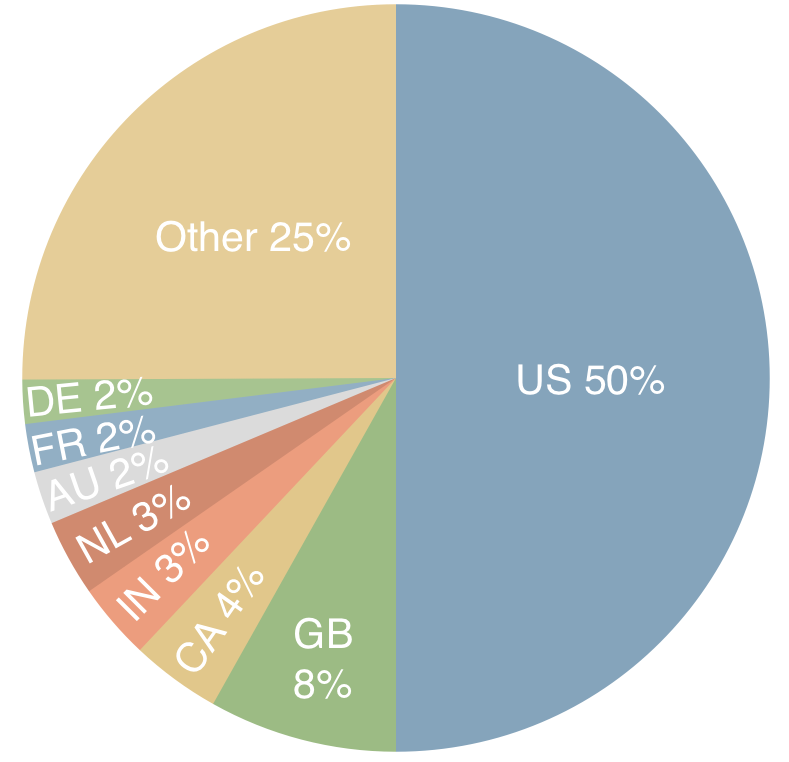
\includegraphics[scale=0.3]{companyCountries.png}
\centering
\caption{Distribution of companies per country (Total 236,235 companies)}
\label{fig:countryDistribution}
\end{figure}


\subsubsection{Dataprocessing}
Because both sources have different advantages and information and as mentioned in the last section a different structure,
it makes sense to combine both datasets into one, that covers all the necessary information needed for clustering,
and has one defined dataschema.

The biggest challenge in combining these two datasets is finding the right corresponding company in the respectively
other dataset.
The used approach was to join to datasets on an equal string match of both company names. If companies have slightly different names
in both sets, they will be matched if they have the same website url given. Otherwise a new entry will be created in
the resulting dataset. This resulted in a dataset of 236,235 companies. As you can see in Figure \ref{fig:countryDistribution}
the most companies are located in the United States. Since both datasources are US-companies and the main users are therefore
from the united states that distribution is not surprising. The overall dataset contains companies from 220 countries.


\subsubsection{Used data for clustering}
\label{dataSubset}
Because this thesis looks for correlation between company characteristics and the company's demands, we can only use companies
we also have demand information for. So we compared the existing posts from the NoiseToOppotunity\cite{n2o} database with
the crawled companies from LinkedIn and Crunchbase. This resulted in a test dataset of 1129 companies.

% Challenge: Finding a combination of Features which matches the closeness of companies
% to the need's development
\subsection{Company Features}
\label{companyFeatures}
Features are variables or a combination of variables that can describe certain characteristics of an entity. Using the right
features is essential to prove that strongly related businesses develop similar product needs. In this case the features have
to describe characteristics that influence a companies buying behaviour.

Regarding to Porter \cite{CompanyClusters} a company's \emph{location} has a high influence on how it acts. Companies will often rather know what happens next to
them than at a totally different place. Steps taken by companies right next to each other will have a higher impact on
how each of them reacts to particular circumstances, especially purchases made by one of the companies may lead to an economic
advantage. Other companies are then forced to close this gap by doing similar purchases.

Of course the location is important but has less impact if the companies next to each other do not compete somehow.
Referring to Porter \cite{CompanyClusters} companies of the same \emph{industry} are often shaped in clusters at one location.
They are using the same infrastructure and increasing the clusters know how.

So the first two features that cause the highest influence from one company to another are a company's location and its industry.

An increasing number of employees within a company leads to a higher complexity. Also bigger companies have other needs and higher expenses than
smaller ones have. Therefore companies of similar size are more related to each other than to smaller sized companies.
This leads us to the third feature, a company's size measured by its \emph{number of employees}.

According to Webster and Wind \cite{BusinessBuyingBehavior} companies are exposed to 6 different influences. These influences are already covered
by the selected features. For example by selecting a company's location the legal, economic and political influences which
are the strongest ones are considered.

Other characteristics mentioned in chapter 4.1 and displayed in figure \ref{fig:sourcesSchemas} could also be used as features. But as the selected 3 features cover all the aspects
discussed during the economic background, we stick to the three features \emph{location}, \emph{industry}, \emph{number of employees}. A comparison of results using different combinations of
features could be part of future work. This thesis focuses on finding a correlation between this features and the company's demand
demand-evolvement.


\subsection{Calculate Proximity}
\label{companyProximity}
The calculation is performed on the set described in section \ref{dataSubset}, that contains 1129 documents. This would result in a maximum count of
realtionships of 636.756, where each company has a relationship to each other, but not itself. Thats the result of following
function where n equals the number of companies.

\begin{center}
  { \Large #relations \LARGE = $\frac{n*(n-1)}{2}$}
\end{center}

For the proximity we take all of the features and weight them according to their influence. Regarding to the conclusions in chapter
\ref{companyFeatures} we assume that location and industry have a high weight whereas the company size does not have that much impact
on a company's buying behaviour.

The calculation takes two companies and compares the defined features. We check for an industry match $I_m$, whether both companies have at least
one common industry, for a location match $L_m$, whether both companies have at least one office in the same city or country, and finally
for and employees count match $E_m$, whether both companies have the same employees range. If a match exists the corresponding
value is one otherwise it is zero.

\begin{center}
  \label{proximityFormula}
  {  proximity = $1 - ( I_w * \frac{I_m}{I_w + L_w + E_w} + L_w * \frac{L_m}{I_w + L_w + E_w} + E_w * \frac{E_m}{I_w + L_w + E_w})$}
\end{center}

The proximity formula, with $E_w$ for the company's size weight, $L_w$ for the company's location weight and $I_m$ for the company's
industry weight return a value between zero and one. The smaller the value the closer 2 companies are.

\subsection{Cluster scoring}
\label{clusterScoring}
Annahme: Jede Company entwickelt nur ein demand / What clustering algorithm used? What exactly? cluster company level -> Partition

To be able to evaluate which feature weight works best and which partitions of the ones formed by the
clusterings it is necessary to have some characteristics to compare.

The first and most important one is the function score(X) that calculates how good a cluster is according to the fact whether
it strongly develops only a demand for one specific product.

\begin{figure}[ht]
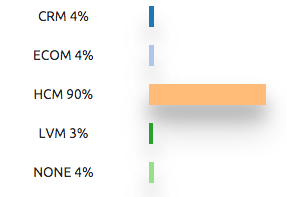
\includegraphics[scale=0.6]{goodCluster.png}
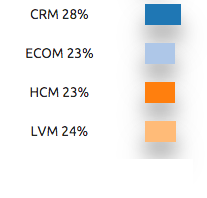
\includegraphics[scale=0.6]{badCluster.png}
\centering
\caption{A good and a bad example of a cluster's demand development}
\label{fig:clusterDemandDevelopment}
\end{figure}

Figure \ref{fig:clusterDemandDevelopment} shows a good demand development on the left and a bad one on the rigth. The used dataset
of demand-posts covers 5 different products: CRM, ECOM, HCM and LVM. The percentage value says how many of the companies within
the according cluster raised a demand of the corresponding product.
The left distribution reveals that the remaining companies in the cluster may also be interested in a HCM product.

A good distribution can be recognized easily as human beings. But we do not want to have a closer look  at each
product distribution to decide wether a partition is good or bad.
In order to process each cluster combination using we developed a function to
distinguish between bad and good product distributions.

\begin{figure}[ht]
  {
    \Large Let $ X \subseteq \mathbb{Q},
    score(X) = \frac{ maxVal( ( max2(X) - avg2(X) ), 1 ) }{ ( max(X) - avg(X) ) }$ \newline \newline
    $max(X) =  $ \large maximum value of set X \newline
    $avg(X) =  $ \large average value of set X \newline
    $max2(X) =  max( X \textbackslash \{ y | y = max(X)\} )$ \newline
    $avg2(X) =  avg( X \textbackslash \{ y | y = max(X)\} ) $ \newline
    \large Let $k,l \in \mathbb{Q},$ $maxVal(k,l) =$  \large returns the bigger value \newline
  }
  \centering
  \caption{The scoring function}
  \label{fig:scoringFunction}
\end{figure}

The function score(X) returns a value that describes the ratio between the difference of the highest value and the
average to the difference of the second highest value and the average without the highest value. The closer the value
is to 0 the better the cluster.

If the highest value strongly differs from all the others than it has a high difference to the average value.
If the highest value is by far the highest than the difference between the second highest value and the average without
the higest value will small. To prevent a wrong result the denominator has to be at least 1 because otherwise the
whole value could be 0 even if the highest value does not have a high difference to the average.

To clarify the formula we are going to calculate for the two examples in figure \ref{fig:clusterDemandDevelopment}
The Left distribution:
\begin{center}
  score([4,4,90,3,4]) =  {\Large $\frac{ maxVal( ( 4 - 3,75 ), 1 ) }{ ( 90 - 21 ) } = \frac{ 1 }{ 69 } =$} 0.0144 \\
\end{center}

The right distribution:
\begin{center}
  score([28,23,23,24,6]) =  {\Large $\frac{ maxVal( ( 24 - 19 ), 1 ) }{ ( 28 - 20,8 ) } = \frac{ 5 }{ 7,2 } =$} 0.6944 \\
\end{center}


The left distribution has as expected a better value than the right distribution. To evaluate a whole cluster combination
the rating for each cluster gets calculated. All the ratings will then be averaged according to the clusters size.
So a good rating within a small cluster will not have as much impact as a good rating in a bigger sized cluster.

Other measurments to value a cluster combination are the total number of companies within the clusters or the
highest average of a products demand. The more companies covered, the more efficient the demand predictions are.
Also the higher the average covering is for the products, the more actively are the companies spreading demands
within a cluster. An average covering takes only the highest coverage from each of the existing clusters and averages
them. According to our exmaple in figure \ref{fig:clusterDemandDevelopment} we would calculate the average of 90 and 28.

\subsection{Downsides}
As we simplified our approach by assuming that every company raises one product demand only, we have also have to
consider what happens if companies also raise more than one demand, which is the more realistic case.

The assumption allowed us to use an exclusive clustering algorithm. So if companies raise more demands they have
to be in more than one cluster according to their demand. This allows us to still be able to use the same scoring function
but it would support multiple demands per company.

This would require a fuzzy algorithm. C-Means could be used for this task. It is an extension of the standard kMeans
algorithm and was first introduced by Bezdek \cite{fuzzyClustering}. This implementation could be part of the future work.






















% {\small
% \begin{tabular}{ccccccc}
%   Clusters & Avg Rating & Level & High Avg & Big Cluster & Weight Sz In Lo & Tree depth \\
%     5 & 0.7969 & 28 & 38\% & 1049 & 0,0,1 & 777 \\
%     6 & 0.9860 & 67 & 22\% & 217 \(561\) &  1,0,0 & 284 \\
%     6 & 0.9860 & 67 & 22\% & 217 \(561\) &  0,0,1 & 284 \\
%     6 & 0.7001 & 47 & 48\% & 12 \(34\) & 1,1,1 & 59 \\
%     8 & 0.7375 & 51 & 45\% & 10 \(42\) & 2,4,1 & 61 \\
%     8 & 0.8693 & 41 & 47\% & 9 \(39\) & 2,2,1 & 50 \\
%     5 & 0.7125 & 10 & 39\% & 1086 \(1097\) & 2,8,1 & 63 \\
% \end{tabular}
% }
